% Chapter 1

\chapter{Classic percolation}

\label{ch:classicpercolation} % For referencing the chapter elsewhere, use \autoref{ch:introduction}

%----------------------------------------------------------------------------------------

%----------------------------------------------------------------------------------------

\section{Basic definitions}

We begin with a graph G representing a slattice of size $L$ in $d$ dimensions, such that $|G| = L^d$.
Each node in the graph is independently set to be "alive"/"white" with probability $p$ and "dead"/"black" with probability $1-p$. $p$ is often called the occupation probability.
Our goal is to study the properties of the lattice after this "coloring" has taken place. This is what such a lattice looks like: (IMAGE)


\begin{defn}
A cluster is a set of white connected nodes in the graph.
\end{defn}


\begin{defn}
A lattice is said to have percolated if there exists a macroscopic cluster, i.e. a cluster which spans the whole lattice.
\end{defn}

For the case of $d<\inf$, one can (arbitrarily) pick a dimension $i$ from ${1, 2, ... d}$ and use it as the defining dimension for percolation, i.e. a lattice has percolated if there exists a cluster that intersects both boundaries of the lattice. For $d=2$, for example, we can use the convention that a lattice has percolated if there is a cluster that connects the top boundary and the bottom boundary (left-right would be equally good).

The process is, of course, random. So we define an indicator random variable $H_{p,L}$ which represents whether a particular lattice has percolated:

\begin{defn}
\[
	H_{p,L} =
    \begin{dcases}
        1 & \text{if lattice has percolated} \\
        0 & \text{otherwise} \\
    \end{dcases}
\]
\end{defn}
As we shall see, percolation models are the simplest models that exibit a phase transition, meaning that there exists a particular occupation probability $p_c$ at which the behavior of the system is expected to change dramatically. This change will be reflected in a number of quantities of interest which will study in the next sections.
As we vary $p$, larger and larger clusters are expected to form. However, in the case that $L < \inf$ and $p < 1$, there is always a possibility that no percolating cluster will be observed (i.e even if $p = 0.999$ there is a non-zero probability all nodes are dead).

\begin{defn}
$\Pi_{p,L} = \E[H_{p,L}]$ is the probability that a particular lattice will percolate.
\end{defn}

As we increase $L$, the behaviour of $\Pi_{p,L}$ as a function of $p$ approach a step function at $p=p_c$. Which means that in the limit of very big L, the lattice percolates with probability 1 for $p > p_c$, and does not percolate with probability 1 for $p < p_c$.

\begin{defn}
The percolation threshold $p_c$ is the occupation probability $p$ such that a percolating cluster exists with probability $1$ on an infinite lattice (that is, in the limit $L \rightarrow \infty $).
\end{defn}

At this point, its not entirely obvious why we choose this particular definition. One could, a priori, choose to define $p_c$ as the probability at which there is a $\frac{1}{2}$ probability that the lattice percolates, for example. Or one could choose to define it in terms of a finite lattice. As we shall see, the definition given above is the only one that is well definited when we start working with multiple dimensions and multiple types of lattices.

\begin{defn}
$P_{p,L}$ is the fraction of nodes belonging to a percolating cluster.
\end{defn}


Next, we'll look at some quantities of interest and study their behavior as a function of $p$, in particular for small values of $|p - p_c|$, i.e. for $p$ close to $p_c$. The reason for studying this particular regime will become apparent later.


\begin{defn}
	$n_{s}(p)$ is the cluster size distribution, i.e the number of s-sized clusters (clusters with s nodes) per lattice size.
\end{defn}

\begin{defn}
$\chi(p)$ is the average cluster size.
\end{defn}

\begin{defn}
	$s_{\xi}(p)$ is the average size of the largest cluster.
\end{defn}

\begin{defn}
$\xi(p)$ is the average linear size of the largest cluster.
\end{defn}



\section{1D Case: toy model}\label{sec:1d}

Our goal now is to better understand the 1D case. It is one of the few percolation models that can be solved analitically, and therefore can give us some insight into the dynamics of the system. Many of the properties exhibited still extend to higher dimensions, if one knows where to look.

\begin{figure}[h]
  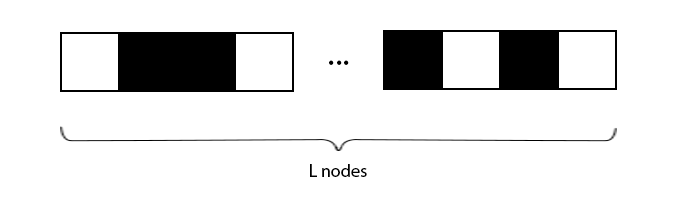
\includegraphics[width=\linewidth]{Images/1dlattice.png}
  \caption{A 1D lattice of size L, with a few dead nodes}
  \label{fig:1dlattice}
\end{figure}

For simplicity, we'll define a new indicator random variable $S_i$ which denotes the state of the i-th node in the lattice. The PMF for $S_i$ is

$$
	S(i) =
    \begin{dcases}
        1 & \text{with probability p} \\
        0 & \text{with probability 1-p} \\
    \end{dcases}
$$

\subsection{Percolation threshold $p_c$}

For a 1D lattice, it is clear that percolation can only happen in a lattice of size $L$ if all nodes in the lattice are dead. Since each coloring is independent, we have that

\begin{equation}
	\begin{split}
		\Pi_{p,L} & = \Pr[S(1) = 1, ... S(L) = 1] \\
				  &	=  \Pr[S(1) = 1]...\Pr[S(L) = 1] \\
				  & =  p^L
	\end{split}
\end{equation}

It is clear that in the limit $L \rightarrow \infty $, if $p < 1$, $\Pi_{p,L} = 0$.
Therefore, we have that

$$
p_c = 1
$$


It is interesting to notice here that if we were to define $p_c$ in any simpler way, its value would depend on the size of the lattice. For example, suppose we chose to define $p_c$ as the smallest $p$ such that
$$
  \Pi_{p,L} \geq \alpha
$$

For some $0 < \alpha < 1$. In other words, if $\alpha$ was $\frac{1}{2}$, that would be equivalent to defining $p_c$ as the smallest $p$ such that the lattice percolates with probability $\frac{1}{2}$. Then we'd have

\[
\begin{split}
  & \Pi_{p,L}  \geq \alpha \\
  & \Rightarrow p^L \geq \alpha \\
  & \Rightarrow p \geq \alpha^{\frac{1}{L}}
\end{split}
\]

We'd like to make our definitions as universal as possible, in particular we'd like our definition to be indepedent of the size of the lattice. The definition we chose previously accomplishes that. We will see more ways in which any other definition fails in the 2D case as well.

\subsection{Cluster size distribution}

The first non-trivial quantity we want to look at is the cluster size distribution, $n_s$. For a given combination ($p$, $L$) of occupation probability and lattice size, $n_s$ describes the number of $s$-clusters - that is, clusters with s nodes - \textit{per lattice site}.

For the 1D case, we can easily find an analytical expression for $n_s$. Let's start by considering a very long lattice (or equivalently, $L \gg s$). In this case, an s-cluster happens if and only if we see a sequence of $s$ black cells enclosed by a white cells at the left and right boundaries. The probability for a white cell is $(1-p)$, and the probability of a black cell is $p$. Therefore, we expect that the probability of seeing an s-cluster somewhere along the lattice is proportional to $(1-p)^2 p^2$. We also expect that by doubling the size of the lattice, we'll see twice as many s-clusters. Therefore, we expect to see
\begin{equation}
  \langle n_s \rangle \propto L (1-p)^2 p^s \label{chap1_clust_size_dist}
\end{equation}

Below, we can see the cluster size distribution obtained from simulations we've run, for various combinations of $p$ and $L$:

\begin{figure}[h]
  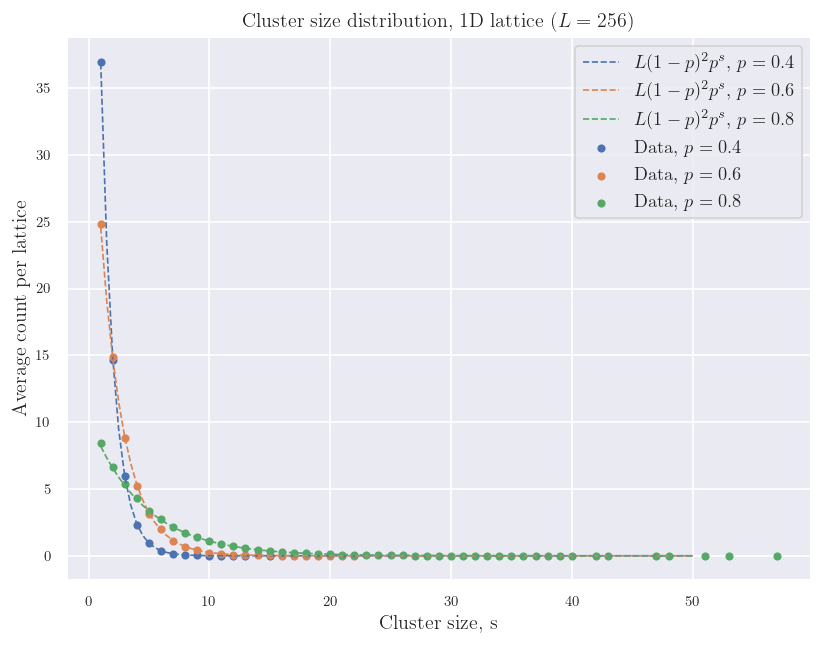
\includegraphics[width=\linewidth]{Images/chap1_clust_size_dist_256.png}
  \caption{Average cluster size distribution in a 1D lattice with $L=256$}
  \label{fig:chap1_clust_size_dist_256}
\end{figure}


\begin{figure}[H]
  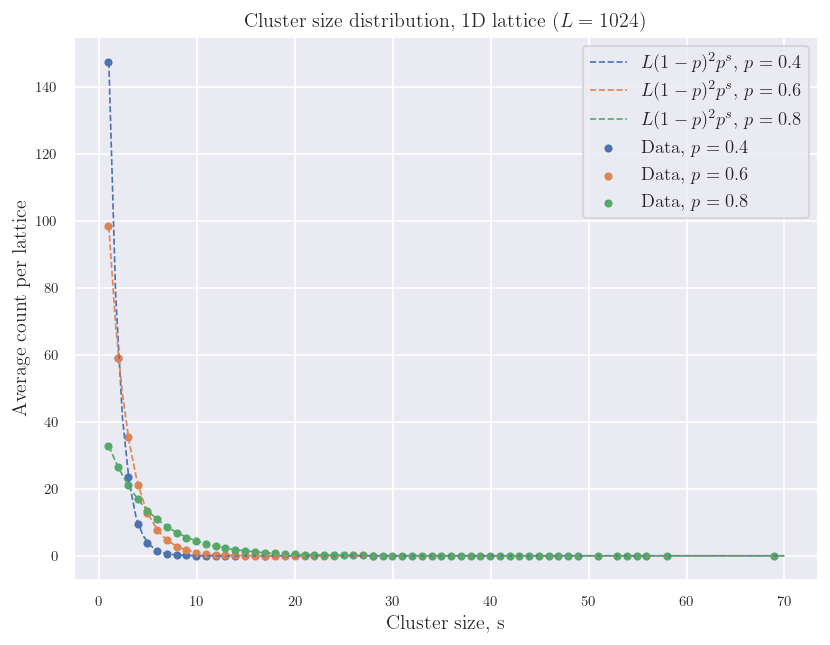
\includegraphics[width=\linewidth]{Images/chap1_clust_size_dist_1024.png}
  \caption{Average cluster size distribution in a 1D lattice with $L=1024$}
  \label{fig:chap1_clust_size_dist_1024}
\end{figure}


One interesting thing to notice is that as we increase $p$, the distribution becomes less pronounced towards smaller clusters. Its easy to see why happens by looking at \eqref{chap1_clust_size_dist}: the ratio of 1-cluster and 2-clusters, for examples, decreases as we increase $p$:

$$
\frac{n_1}{n_2} \propto \frac{1}{p}
$$

Therefore, we expect a bigger difference between $n_1$ and $n_2$ for smaller $p$.

\subsection{Percolating cluster strength}

Next, we'll look at the percolating strength $P(p)$. This quantity  represents the probability that a randomly picked node belongs to the percolating cluster. Another way to think of this quantity is that it represents the fraction of the whole lattice that is covered by the percolating cluster. 

For small values of $p$, all islands are finite. Starting at any randomly site, it is impossible to get arbitrarily far away by walking only along the connected sites. As we increase $p$, the largest cluster becomes infinite at a precise value $p = p_c$. When this happens, it is possible to get arbitrarily far from a starting point in the infinite cluster by walking along the connected sites. For $p < p_c$, there are no infinite clusters, so $P(p)$ vanishes. However, for $p > p_c$, $P(p)$ monotonically increases. For $1 \gg (p - p_c) > 0$, that is, for $p$ greater  but close to $p_c$, we have (REF 1):

$$
    P(p) \propto (p - p_c)^\beta 
$$

The qualitative behaviour of $P(p)$ can be seen in figure (FIG 1)


$\beta$ is a universal critical exponent which depends only on the lattice dimension, and not on its geometry. In 2 dimensions, $\beta = \frac{5}{36}$, is the same for the square, hexagonal, or any other geometry (REF 1)). 

P(p) is one of the order parameters for percolating systems, since it is zero for $p < p_c$, and non-zero for $p > p_c$.

\subsection{Mean cluster size}

Another interesting quantity is $\chi(p)$, the mean cluster size, which is the average number of nodes in among finite clusters. One can think of each node in the cluster as having one "unit of mass", in which case the mean cluster size represents the average mass. Just like $P(p)$, for $\chi(p)$, we have

$$ 
    \chi(p) \propto  |p - p_c|^\gamma \textrm{,} \hspace{0.35cm}  \textrm{for} \hspace{0.15cm} |p - p_c| \ll 1 
$$ 

The qualitative behaviour of $\chi(p)$ can be seen in (FIG 2).


Again, analogously to the percolating cluster strength $P(p)$, $\gamma$ is a universal critical exponent, in the sense that it's independent of the local geometry, and depends only on the dimension of the lattice. In two dimensions, $\gamma = \frac{43}{18}$. One important difference between $\chi(p)$ and $P(p)$, however, is that $\chi(p)$ scales as $|p - p_c|^\gamma$ for both $p < p_c$ and $p > p_c$. However, the constants of proportionality are different in either side.


\subsection{Correlation function}

The correlation function $g(\vec{r})$ encodes how likely it is that two clusters separated by a displacement vector $\vec{r}$ are part of the same (finite) cluster. In 2D,  based on rotational symmetry and in order to simplify the analysis, one often ignores the vector character of  $\vec{r}$ and studies only $g(r)$, where $r = |\vec{r}|$.

\subsection{Phase transitions}

\subsection{Real space renormalisation}



%----------------------------------------------------------------------------------------


\section{Numerical simulations - 2D square}\label{sec:2dsquare}

\subsection{Percolation probability}


\begin{figure}[H]
  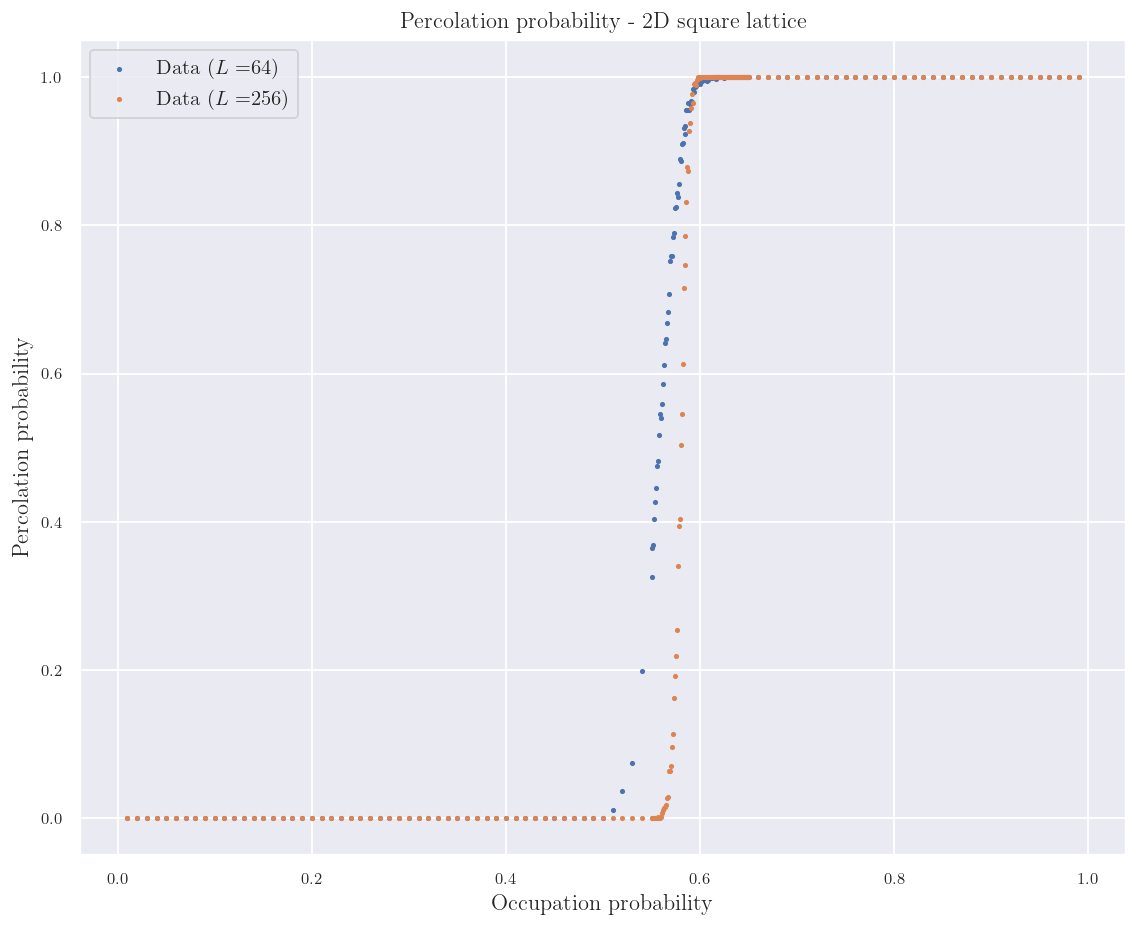
\includegraphics[width=\linewidth]{Images/chap1_perc_prob_1.png}
  \caption{Percolation probability curve for varios lattice sizes}
  \label{fig:chap1_perc_prob_1}
\end{figure}


\begin{figure}[H]
  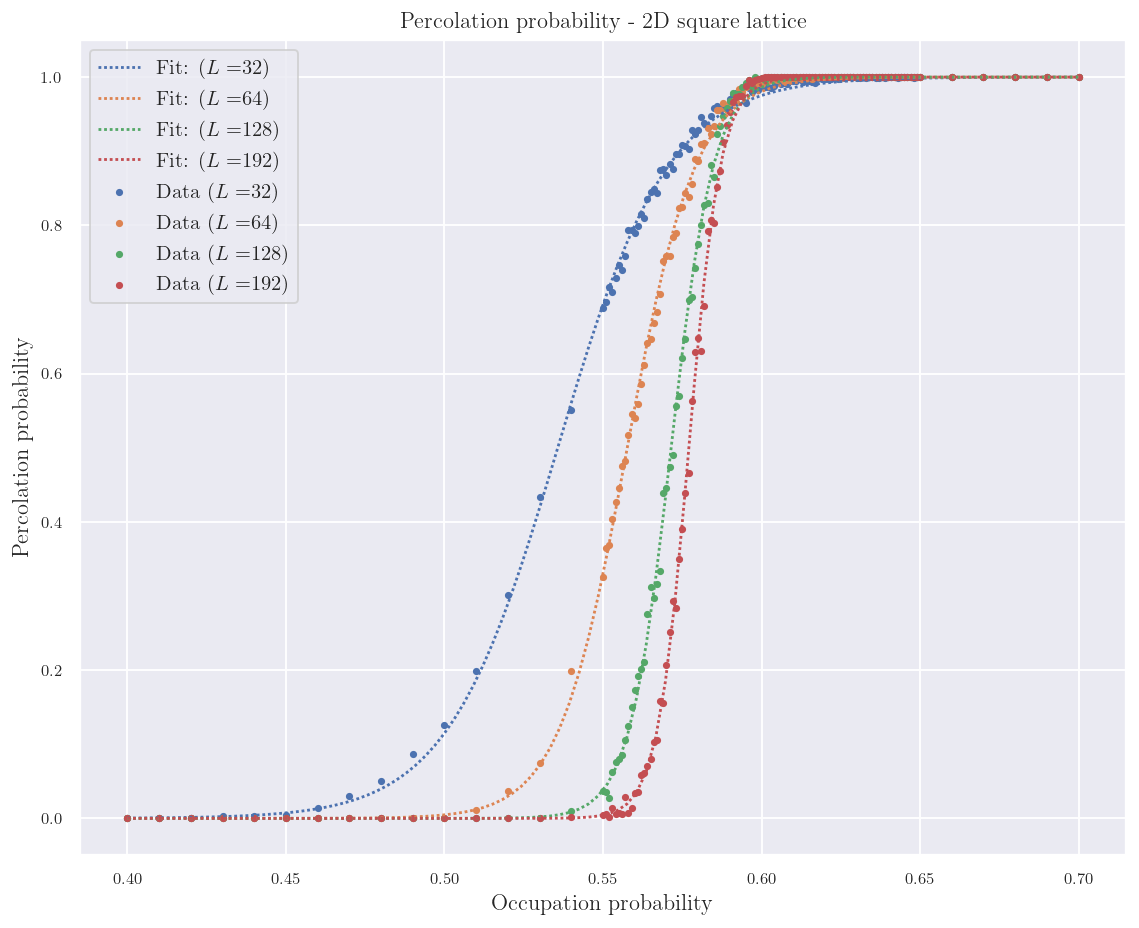
\includegraphics[width=\linewidth]{Images/chap1_perc_prob_2.png}
  \caption{Percolation probability curve zoomed in, along with the sigmoid function best fit}
  \label{fig:chap1_perc_prob_2}
\end{figure}


\begin{figure}[H]
  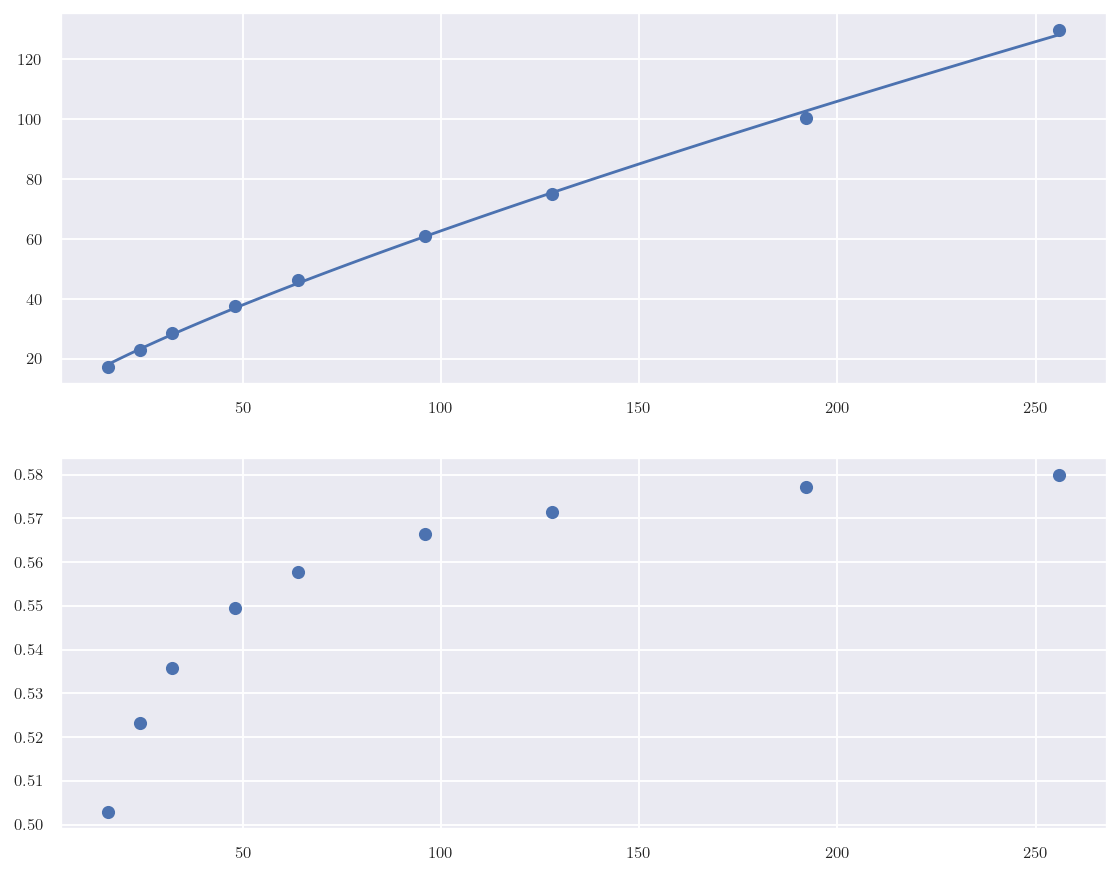
\includegraphics[width=\linewidth]{Images/chap1_perc_prob_3.png}
  \caption{Finite-size scaling analys of the sigmoid function}
  \label{fig:chap1_perc_prob_3}
\end{figure}


\subsection{Mean cluster size}

\begin{figure}[H]
  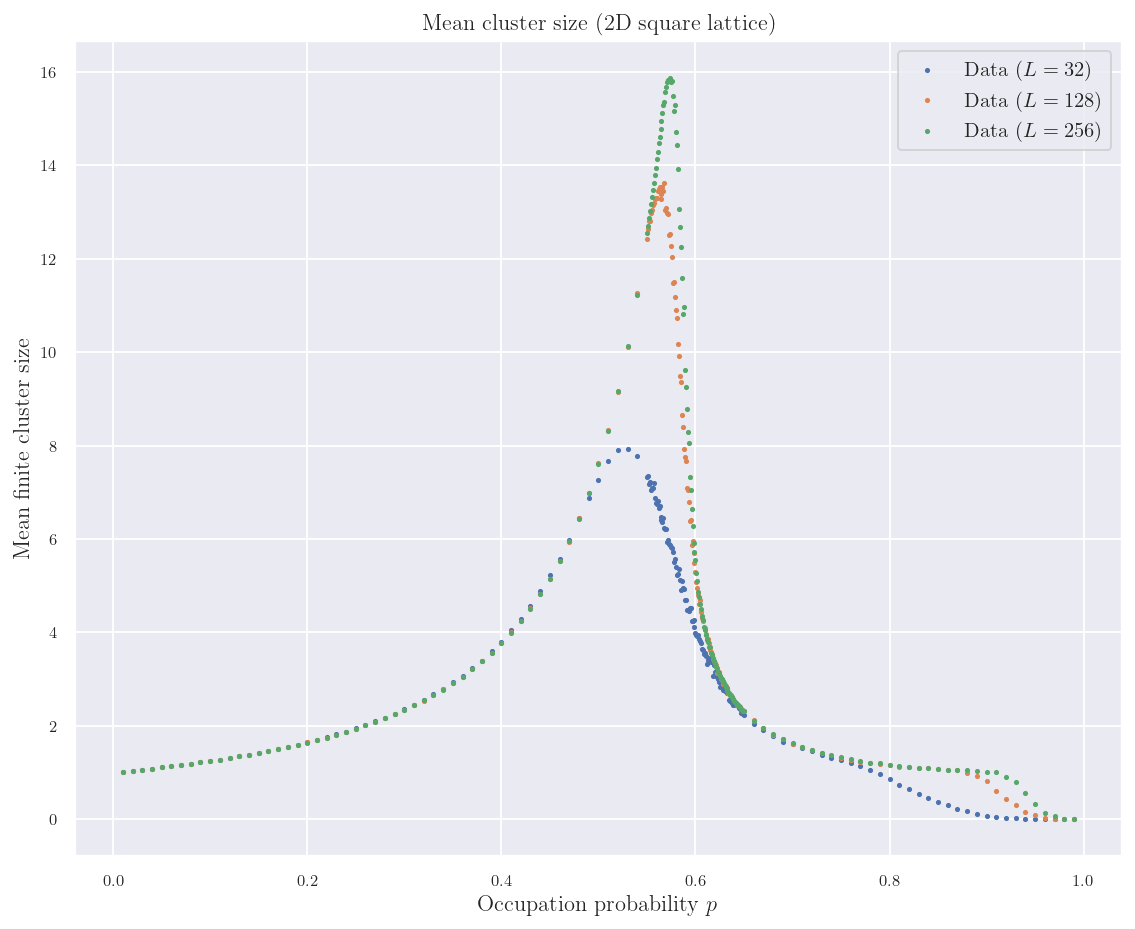
\includegraphics[width=\linewidth]{Images/chap1_mean_cluster_size_1.png}
  \caption{Mean cluster size for various lattice sizes}
  \label{fig:chap1_mean_cluster_size_1}
\end{figure}

\subsection{Percolating cluster strength}


\begin{figure}[H]
  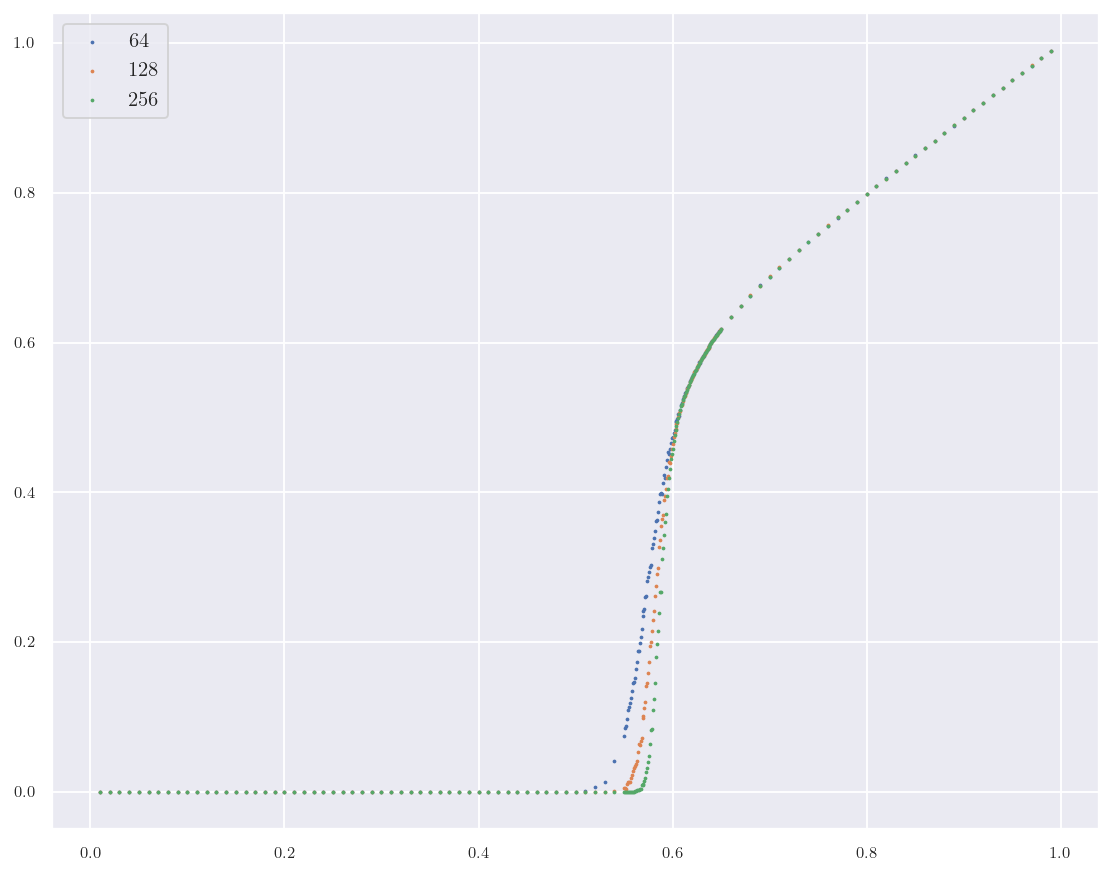
\includegraphics[width=\linewidth]{Images/chap1_perc_clust_strength_1.png}
  \caption{Percolating cluster strength for various lattice sizes}
  \label{fig:chap1_perc_clust_strength_1}
\end{figure}













% \begin{figure}[h]
%   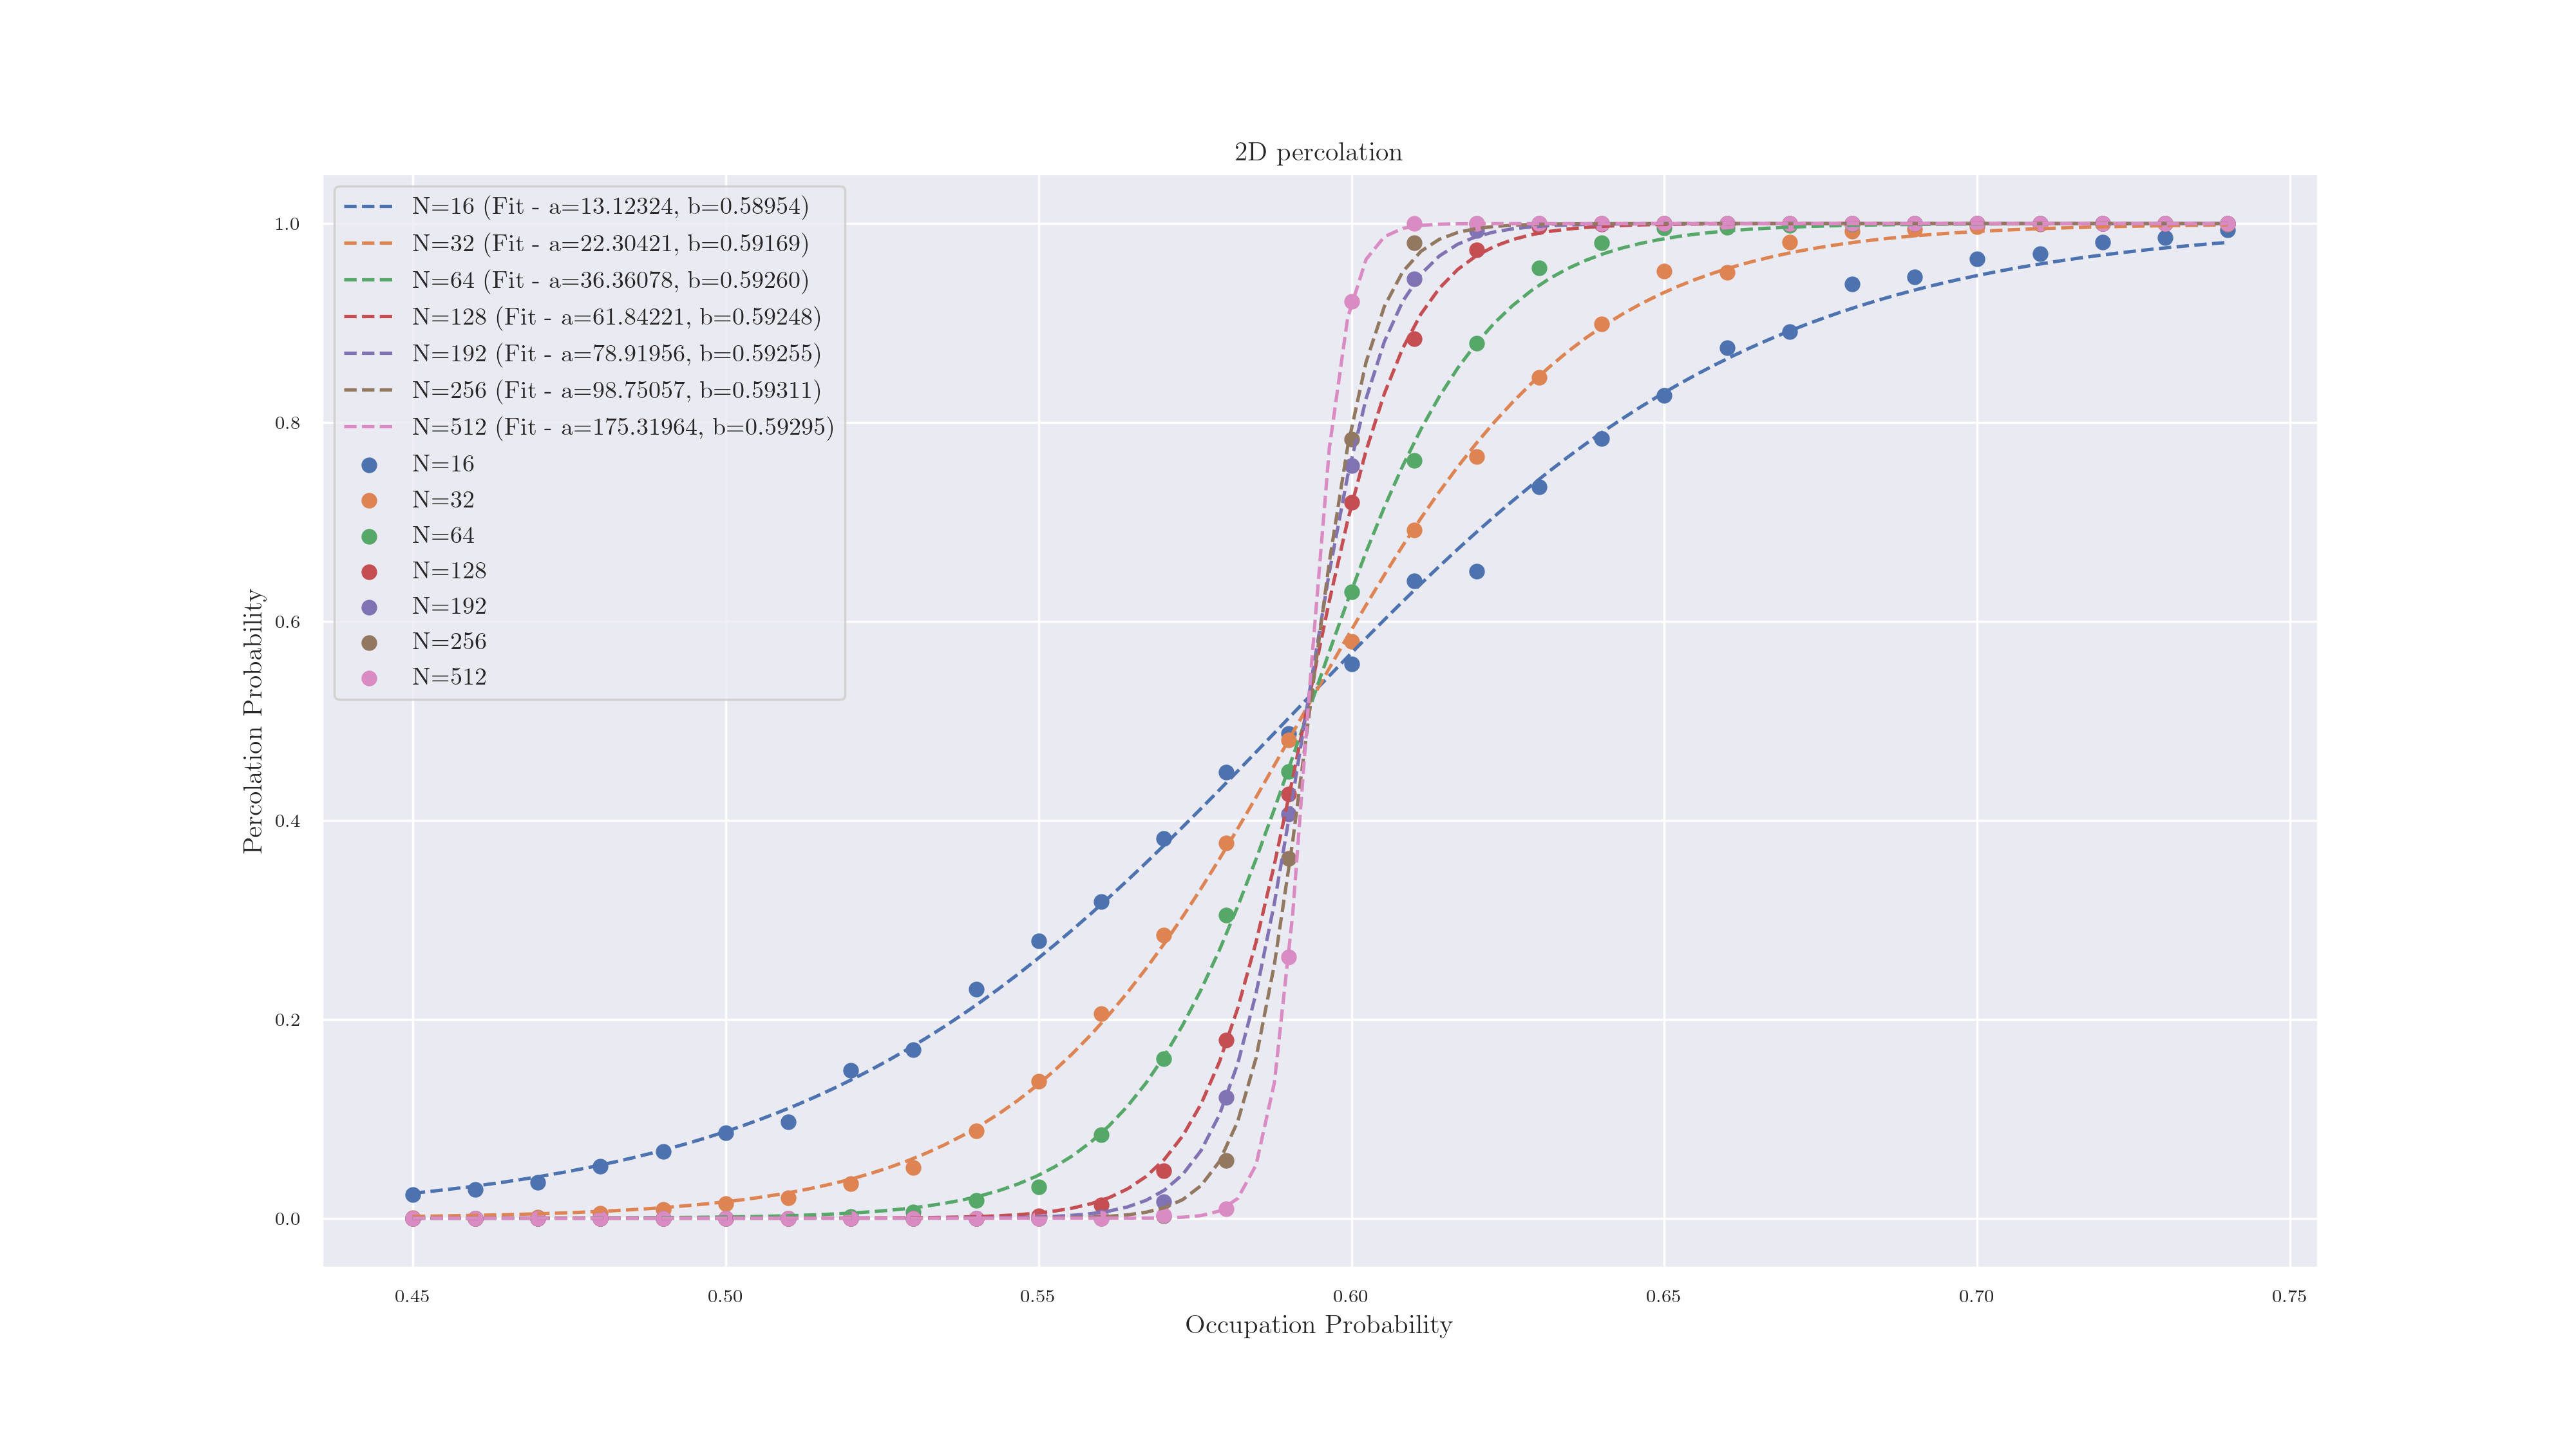
\includegraphics[width=300pt]{Images/perc_2d_prob.png}
%   \caption{Percolation probability for various lattice sizes.}
%   \label{fig:2dlattice_perc_prob}

% \centering%
% \makebox[\textwidth][r]{% %%% you make a box which width is
% %%% not important for the contents of the box itself
% %%% (\textwidth) and which will flush [r] from the right
% %%% ([l] from the left) margin of the text; whatever doesn't
% %%% find place in the box will exceed in the opposite side.
% %%% Please note that a curly brace is still open.
% 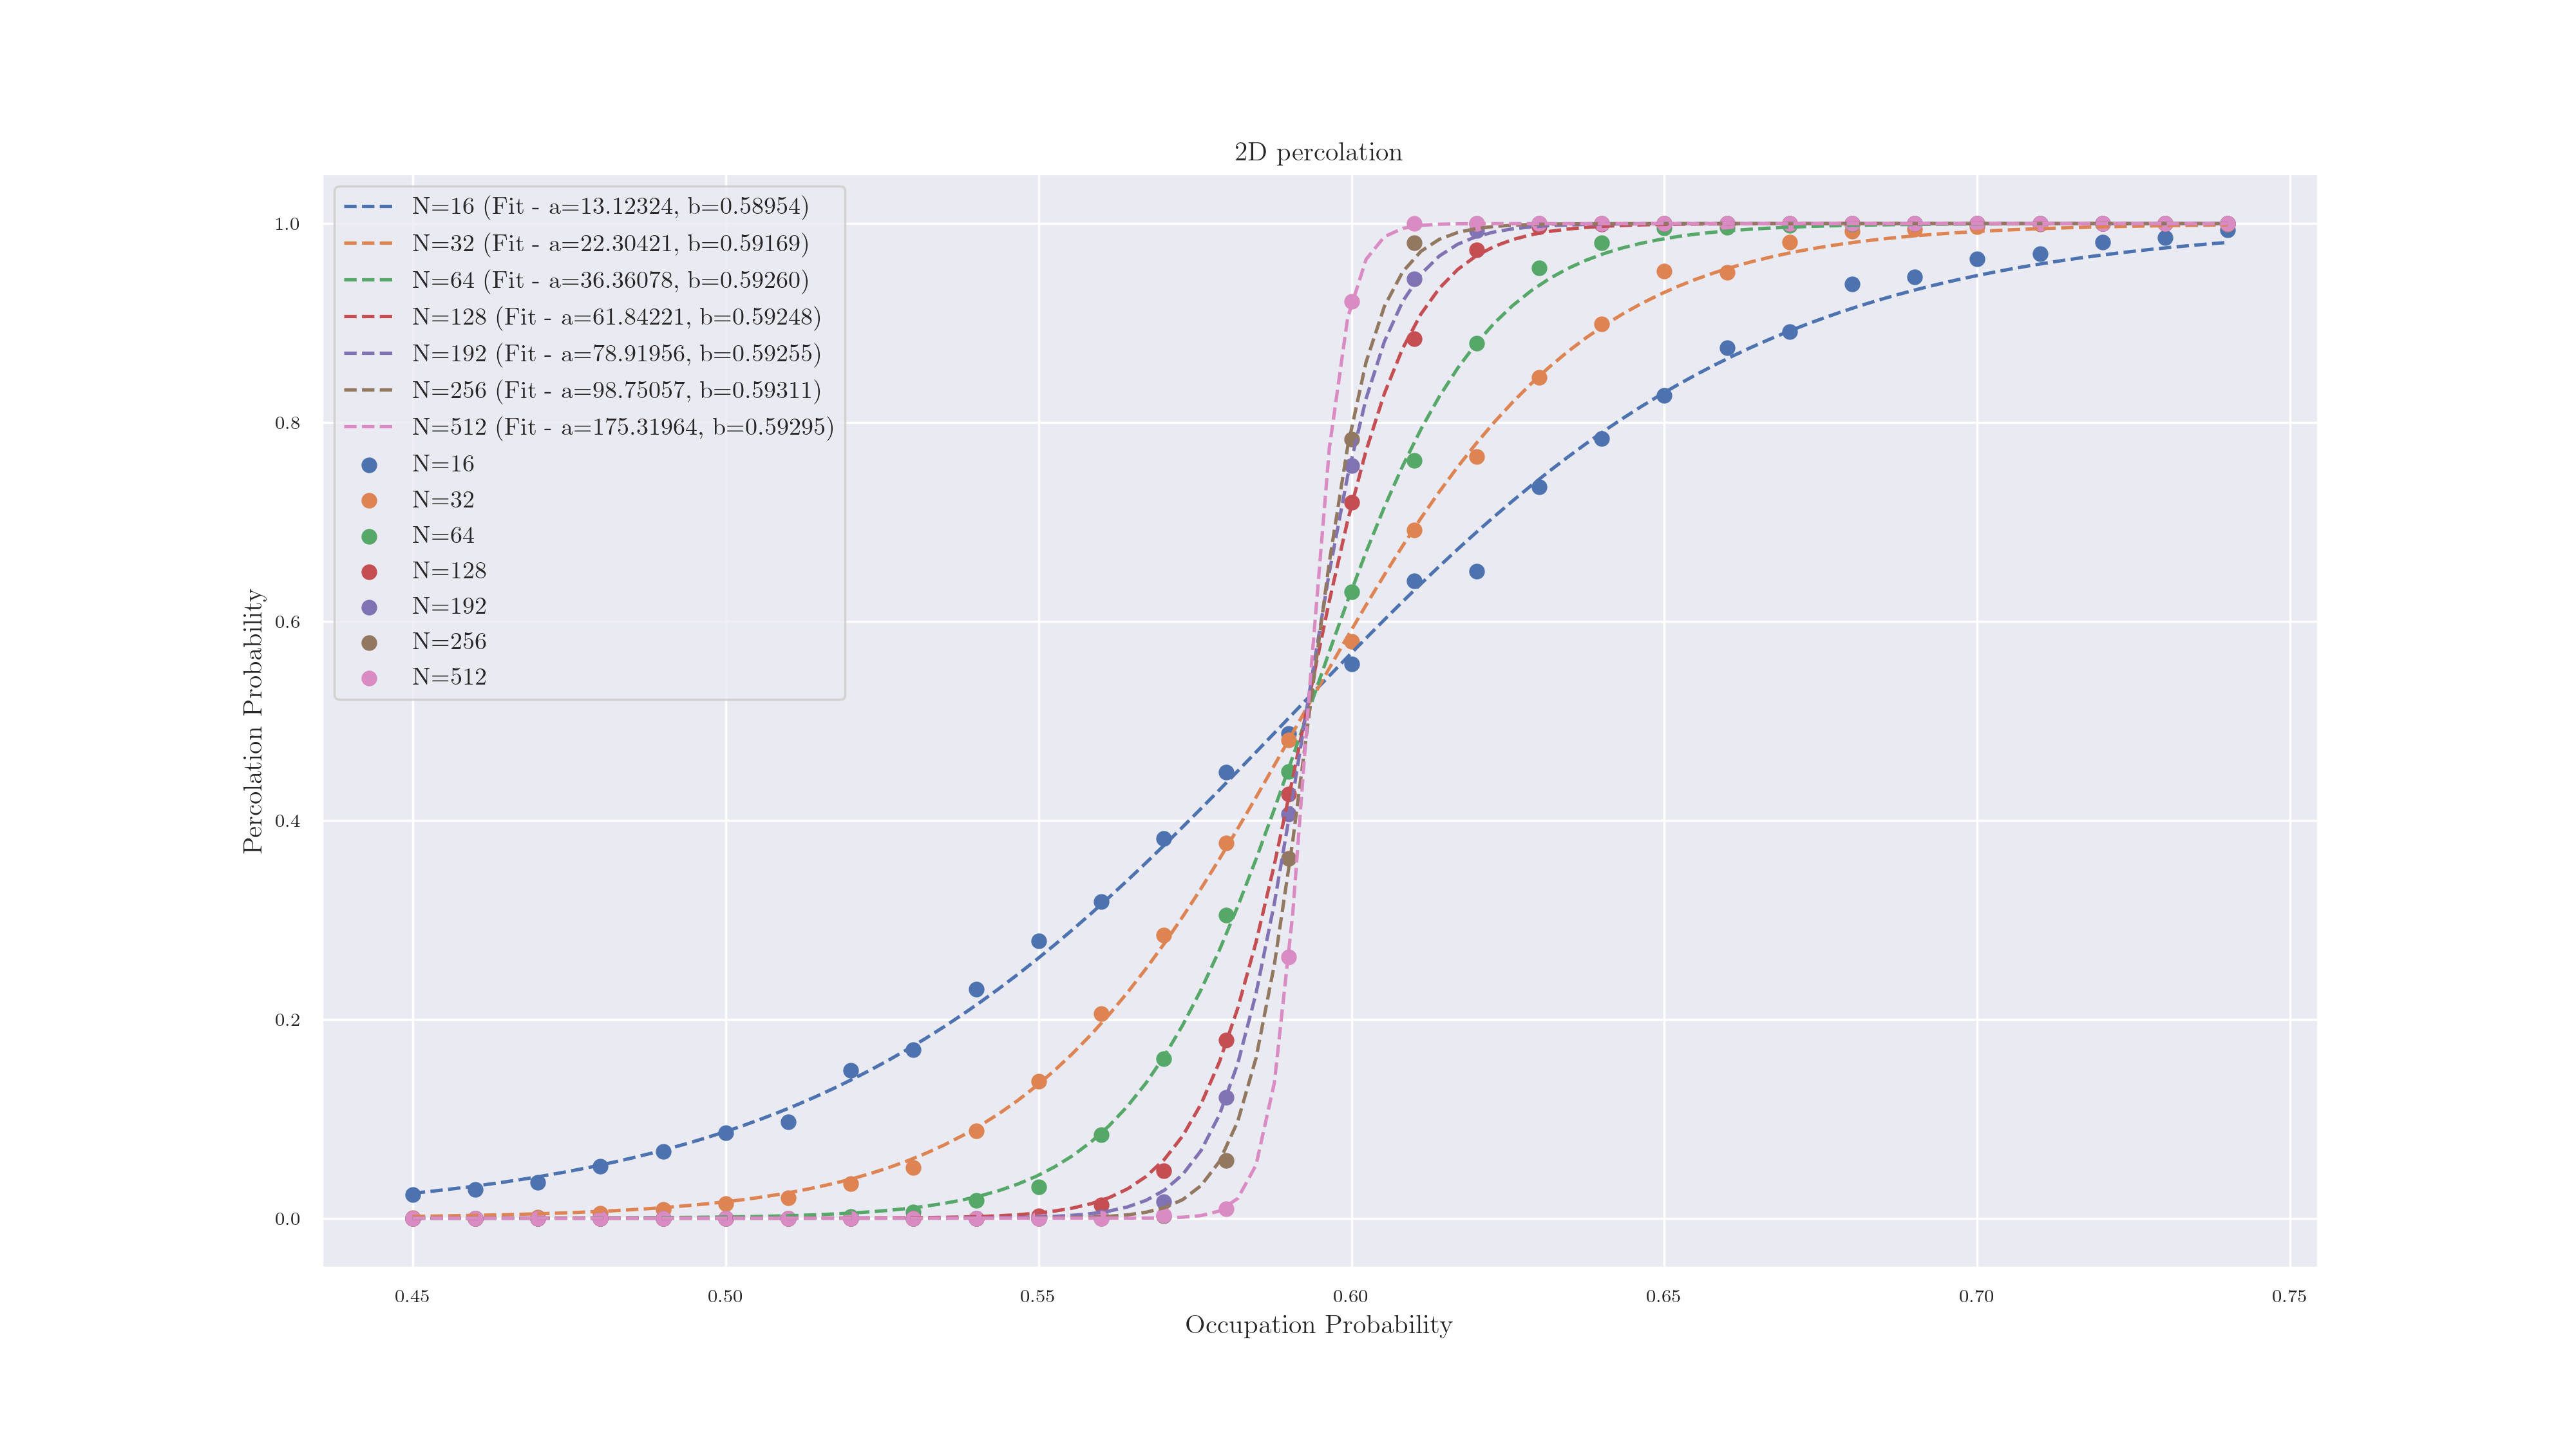
\includegraphics[width=.8\largefigure]{Images/perc_2d_prob.png} %%% you
% %%% can now include your graphic with the usual option for
% %%% \includegrephics
% } %%% Here you "close the box"
% \end{figure}


% \subsection{Critical exponents}

% \subsection{Correlation length}

% \subsection{Phase transitions}

% \subsection{Real space renormalisation}


%----------------------------------------------------------------------------------------

\section{2D in hexagonal lattice}


\section{Bethe lattice}\label{sec:bethelattice}







